\documentclass[11pt,a4paper]{article}

% ----- preamble.tex -----
% % ----- preamble.tex -----
% % ----- preamble.tex -----
% \input{preamble.tex} should be included in all note files before '\begin{document}'
% \lecture{<lectureNumber>: <lectureTopic>}{<mm/dd/yyyy>}{<lecturerName>}{<authorName>}

\hbadness=10000
\vbadness=10000

% page size settings
\setlength{\textheight}{8.5in}
\setlength{\textwidth}{6.0in}
\setlength{\headheight}{0in}
\addtolength{\topmargin}{-.5in}
\addtolength{\oddsidemargin}{-.5in}

% paragraph spacing/indenting settings
\setlength\parindent{0pt}
\setlength\parskip{2.5pt}

% imported packages
\usepackage{amsmath,amssymb,amsthm}
\usepackage{mdframed} % for boxing
\usepackage{graphicx} % for inserting images
\graphicspath{ {./imgs/} }

\usepackage{diagbox} % backslash for tabular/tables
\usepackage{booktabs} % enhances quality of table presentation
\usepackage{tikz}
\usetikzlibrary{arrows,automata,trees,calc}

% ----- \tableofcontents PAGE LINKING (without blue highlight) -----
\usepackage{hyperref}
\hypersetup{
    colorlinks,
    citecolor=black,
    filecolor=black,
    linkcolor=black,
    urlcolor=black
}

% ----- VARIABLE RE-DEFINITIONS -----
\def\epsilon{\varepsilon}
\def\phi{\varphi}


% ----- TODO: MAKE EVERY NEW SECTION START ON NEW PAGE EXCLUDING TOC -----
% \let\oldsection\section
% \renewcommand{\section}{\newpage\oldsection}


% ----- CUSTOM COMMANDS -----
\newcommand{\handout}[5]{
    % \renewcommand{\thepage}{#1-\arabic{page}}
    \noindent
    \begin{center}
        \framebox{
            \vbox{
                \hbox to 5.78in {{\bf CS 4510: Automata and Complexity}\hfill #2}
                \vspace{4mm}
                \hbox to 5.78in {{\Large \hfill #5  \hfill}}
                \vspace{2mm}
                \hbox to 5.78in {{\it #3 \hfill #4}}
            }
        }
   \end{center}
   \vspace*{4mm}
}

\newcommand{\lecture}[4]{\handout{#1}{#2}{Lecturer: #3}{Author: #4}{Lecture #1}}

% keeps contents of the same theorem on the same page
\newcommand{\blocktheorem}[1]{
    \csletcs{old#1}{#1}
    \csletcs{endold#1}{end#1}
    \RenewDocumentEnvironment{#1}{o}{
        % \par\addvspace{cm}
        \noindent\begin{minipage}{\textwidth}
        \IfNoValueTF{##1}{\csuse{old#1}}{\csuse{old#1}[##1]}}{\csuse{endold#1}
        \end{minipage}
        \par\addvspace{0.75cm}
    }
}
\raggedbottom

\theoremstyle{definition}
\newtheorem{example}{Example} % use for example problems
\newmdtheoremenv{definition}{Definition} % use for definitions
\newtheorem{theorem}{Theorem} % use for theorems
\newtheorem{corollary}{Corollary} % use for corollary
\newtheorem{lemma}{Lemma} % use for corollary
\newtheorem{claim}{Claim}

\blocktheorem{example}
\blocktheorem{definition}
\blocktheorem{theorem}
\blocktheorem{corollary}
\blocktheorem{lemma}
\blocktheorem{claim} should be included in all note files before '\begin{document}'
% \lecture{<lectureNumber>: <lectureTopic>}{<mm/dd/yyyy>}{<lecturerName>}{<authorName>}

\hbadness=10000
\vbadness=10000

% page size settings
\setlength{\textheight}{8.5in}
\setlength{\textwidth}{6.0in}
\setlength{\headheight}{0in}
\addtolength{\topmargin}{-.5in}
\addtolength{\oddsidemargin}{-.5in}

% paragraph spacing/indenting settings
\setlength\parindent{0pt}
\setlength\parskip{2.5pt}

% imported packages
\usepackage{amsmath,amssymb,amsthm}
\usepackage{mdframed} % for boxing
\usepackage{graphicx} % for inserting images
\graphicspath{ {./imgs/} }

\usepackage{diagbox} % backslash for tabular/tables
\usepackage{booktabs} % enhances quality of table presentation
\usepackage{tikz}
\usetikzlibrary{arrows,automata,trees,calc}

% ----- \tableofcontents PAGE LINKING (without blue highlight) -----
\usepackage{hyperref}
\hypersetup{
    colorlinks,
    citecolor=black,
    filecolor=black,
    linkcolor=black,
    urlcolor=black
}

% ----- VARIABLE RE-DEFINITIONS -----
\def\epsilon{\varepsilon}
\def\phi{\varphi}


% ----- TODO: MAKE EVERY NEW SECTION START ON NEW PAGE EXCLUDING TOC -----
% \let\oldsection\section
% \renewcommand{\section}{\newpage\oldsection}


% ----- CUSTOM COMMANDS -----
\newcommand{\handout}[5]{
    % \renewcommand{\thepage}{#1-\arabic{page}}
    \noindent
    \begin{center}
        \framebox{
            \vbox{
                \hbox to 5.78in {{\bf CS 4510: Automata and Complexity}\hfill #2}
                \vspace{4mm}
                \hbox to 5.78in {{\Large \hfill #5  \hfill}}
                \vspace{2mm}
                \hbox to 5.78in {{\it #3 \hfill #4}}
            }
        }
   \end{center}
   \vspace*{4mm}
}

\newcommand{\lecture}[4]{\handout{#1}{#2}{Lecturer: #3}{Author: #4}{Lecture #1}}

% keeps contents of the same theorem on the same page
\newcommand{\blocktheorem}[1]{
    \csletcs{old#1}{#1}
    \csletcs{endold#1}{end#1}
    \RenewDocumentEnvironment{#1}{o}{
        % \par\addvspace{cm}
        \noindent\begin{minipage}{\textwidth}
        \IfNoValueTF{##1}{\csuse{old#1}}{\csuse{old#1}[##1]}}{\csuse{endold#1}
        \end{minipage}
        \par\addvspace{0.75cm}
    }
}
\raggedbottom

\theoremstyle{definition}
\newtheorem{example}{Example} % use for example problems
\newmdtheoremenv{definition}{Definition} % use for definitions
\newtheorem{theorem}{Theorem} % use for theorems
\newtheorem{corollary}{Corollary} % use for corollary
\newtheorem{lemma}{Lemma} % use for corollary
\newtheorem{claim}{Claim}

\blocktheorem{example}
\blocktheorem{definition}
\blocktheorem{theorem}
\blocktheorem{corollary}
\blocktheorem{lemma}
\blocktheorem{claim} should be included in all note files before '\begin{document}'
% \lecture{<lectureNumber>: <lectureTopic>}{<mm/dd/yyyy>}{<lecturerName>}{<authorName>}

\hbadness=10000
\vbadness=10000

% page size settings
\setlength{\textheight}{8.5in}
\setlength{\textwidth}{6.0in}
\setlength{\headheight}{0in}
\addtolength{\topmargin}{-.5in}
\addtolength{\oddsidemargin}{-.5in}

% paragraph spacing/indenting settings
\setlength\parindent{0pt}
\setlength\parskip{2.5pt}

% imported packages
\usepackage{amsmath,amssymb,amsthm}
\usepackage{mdframed} % for boxing
\usepackage{graphicx} % for inserting images
\graphicspath{ {./imgs/} }

\usepackage{diagbox} % backslash for tabular/tables
\usepackage{booktabs} % enhances quality of table presentation
\usepackage{tikz}
\usetikzlibrary{arrows,automata,trees,calc}

% ----- \tableofcontents PAGE LINKING (without blue highlight) -----
\usepackage{hyperref}
\hypersetup{
    colorlinks,
    citecolor=black,
    filecolor=black,
    linkcolor=black,
    urlcolor=black
}

% ----- VARIABLE RE-DEFINITIONS -----
\def\epsilon{\varepsilon}
\def\phi{\varphi}


% ----- TODO: MAKE EVERY NEW SECTION START ON NEW PAGE EXCLUDING TOC -----
% \let\oldsection\section
% \renewcommand{\section}{\newpage\oldsection}


% ----- CUSTOM COMMANDS -----
\newcommand{\handout}[5]{
    % \renewcommand{\thepage}{#1-\arabic{page}}
    \noindent
    \begin{center}
        \framebox{
            \vbox{
                \hbox to 5.78in {{\bf CS 4510: Automata and Complexity}\hfill #2}
                \vspace{4mm}
                \hbox to 5.78in {{\Large \hfill #5  \hfill}}
                \vspace{2mm}
                \hbox to 5.78in {{\it #3 \hfill #4}}
            }
        }
   \end{center}
   \vspace*{4mm}
}

\newcommand{\lecture}[4]{\handout{#1}{#2}{Lecturer: #3}{Author: #4}{Lecture #1}}

% keeps contents of the same theorem on the same page
\newcommand{\blocktheorem}[1]{
    \csletcs{old#1}{#1}
    \csletcs{endold#1}{end#1}
    \RenewDocumentEnvironment{#1}{o}{
        % \par\addvspace{cm}
        \noindent\begin{minipage}{\textwidth}
        \IfNoValueTF{##1}{\csuse{old#1}}{\csuse{old#1}[##1]}}{\csuse{endold#1}
        \end{minipage}
        \par\addvspace{0.75cm}
    }
}
\raggedbottom

\theoremstyle{definition}
\newtheorem{example}{Example} % use for example problems
\newmdtheoremenv{definition}{Definition} % use for definitions
\newtheorem{theorem}{Theorem} % use for theorems
\newtheorem{corollary}{Corollary} % use for corollary
\newtheorem{lemma}{Lemma} % use for corollary
\newtheorem{claim}{Claim}

\blocktheorem{example}
\blocktheorem{definition}
\blocktheorem{theorem}
\blocktheorem{corollary}
\blocktheorem{lemma}
\blocktheorem{claim}

\begin{document}
\lecture{EXAM 1: Compiled Notes (Lecture 1-8)}{08/23/2022-09/15/2022}{Zvi Galil}{Austin Peng}
\tableofcontents

% TODO: how do i fix this to have new page before every section, but not before the table of contents
\AddToHook{cmd/section/before}{\newpage}

% -----------------------------
% START OF LECTURE 1
% -----------------------------

\section{Lecture 1: Introduction}
\subsection{Topics To Be Familiar With:}
\subsubsection{Sets}
\begin{itemize}
    \item sets are elements drawn from some universe:
    \begin{itemize}
        \item $\mathbb{Z}$ (integers)
        \item $\mathbb{N}$ (natural numbers)
        \item $\mathbb{R}$ (real numbers)
        \item $\mathbb{C}$ (complex numbers)
    \end{itemize}
    \item set operations:
    \begin{itemize}
        \item union: $A \cup B$
        \item intersection: $A \cap B$
        \item complement: $\overline{A}$
        \item Cartesian product: $A \times b$ (pairs)
        \item power: $A^k$ (k-tuples)
    \end{itemize}
\end{itemize}

\subsubsection{Functions}
\begin{itemize}
    \item functions are mappings from one set to another:
    \begin{itemize}
        \item $f: D \rightarrow R$
        \subitem $f(x) = x^2$
        \item $f: Z \times Z \rightarrow Z $
        \subitem $f(x,y) = x + y$
    \end{itemize}
\end{itemize}

\subsubsection{Relations}
\begin{itemize}
    \item relation $R$ can be written as $xRy$
    \begin{itemize}
        \item \textbf{reflexive}: $xRx$
        \item \textbf{symmetric}: $xRy \implies yRx$
        \item \textbf{transitive}: $xRy \text{ and } yRz \implies xRz$
        \item \textbf{equivalence}: if relation R is reflexive, symmetric, and transitive
    \end{itemize}
\end{itemize}

\subsubsection{Graphs}
\begin{itemize}
    \item a graph $G=(V,E)$ has vertices $V$ and edges $E$
    \item a graph may be directed or undirected
\end{itemize}

\subsubsection{Strings}
\begin{itemize}
    \item "abc" is a string
    \item a string is a sequence of symbols from an alphabet $\Sigma$
    \item $\Sigma^*$ is the set of all strings over $\Sigma$
    \item $\Sigma^*$ contains the empty string $\epsilon$, all strings of length 1, all strings of length 2, etc.
\end{itemize}

\subsubsection{Boolean Logic}
\begin{itemize}
    \item 3 main operations: "and" ($\land$), "or" ($\lor$), "not" ($\lnot$)
    \item these operations are performed on variables and constants (true and false)
\end{itemize}

\subsubsection{Proofs}
\begin{itemize}
    \item mathematics consists of definitions, statements/lemmas/theorems, and proofs
    \item 3 common types of proofs:
    \begin{itemize}
        \item proof by construction
        \item proof by contradiction
        \item proof by induction
    \end{itemize}
    \item these operations are performed on variables and constants (true and false)
\end{itemize}

\subsection{Finite Automata and (Regular Languages)}
Consider an automatic door with the inputs $\{\text{F(ront)}, \text{N(either)}, \text{B(oth)}, \text{R(ear)}\}$.
The door has 2 states: open and closed. The door will only open if there is someone in front and not in the rear (door swings inward).
If the door is open, but nobody is there, the door will close.

\begin{tikzpicture}[node distance={3cm}, semithick, main/.style = {draw, circle}]
    \node[state] (0) {closed};
    \node[state] (1) [right of=0] {open};

    % closed
    \path (0) edge [loop left] node {N,B,R} (0);
    \draw[->,out=15,in=165] (0) to node[above] {F} (1);

    % open
    \path (1) edge [loop right] node {F,B,R} (1);
    \draw[->,out=195,in=345] (1) to node[below] {N} (0);
\end{tikzpicture}

\begin{example} $M_1$

    \begin{tikzpicture}[node distance={3cm}, semithick, main/.style = {draw, circle}]
        \node[name=input] {};
        \node[state] (0) [right of=input]{$q_0$};
        \node[state,accepting] (1) [right of=0] {$q_1$};
        \node[state] (2) [right of=1] {$q_2$};

        % q_0
        \draw[->] (input) -- (0);
        \path (0) edge [loop above] node {0} (0);
        \draw[->] (0) to node[above] {1} (1);

        % q_1
        \path (1) edge [loop above] node {1} (1);
        \draw[->,out=15,in=165] (1) to node[above] {1} (2);
        
        % q_2
        \draw[->,out=195,in=345] (2) to node[below] {0, 1} (1);
    \end{tikzpicture}
\end{example}

\begin{itemize}
    \item $q_0$ is the starting state
    \item $q_1$ is the accepting statements
    \item all transitions ($\delta=0,1$) are defined for all states
    \item let x be a binary string $1101$, $M_1$ will accept $x$ because it ends at $q_1$
    \item $L(M_1)=$ all $x$ such s.t $M_1$ accepts $x$ if $x$ has a 1 AND either ends with a 1 or with an even number of 0s
\end{itemize}

\subsubsection{Formal Definition Of A Deterministic Finite Automaton}
\begin{definition}
    A deterministic finite automaton is a 5-tuple $M=(Q, \Sigma, \delta, q_0, F)$ where:
    \begin{itemize}
        \item $Q$ is a finite set called the states
        \item $\Sigma$ is a finite set called the alphabet
        \item $\delta: Q\times\Sigma\rightarrow Q$ is the transition function
        \item $q_0$ is the initial state
        \item $F\subseteq Q$ is the accepting states
    \end{itemize}
    Note: $\delta(q,a)=p$ means that if DFA is in state $q$ and sees $a$, it goes to state $p$
\end{definition}

\newpage
\subsubsection{Formal Definition Of Computation}
\begin{definition}
    A \textbf{computation} of a deterministic finite automaton (DFA) $M$ on an input string $x=x_1,...,x_n\in\Sigma^*$ is a sequence of states $q_0,...,q_n\in Q$ s.t. for $i=0,...,n-1$ $\delta(q_i,x_{i+1})=q_{i+1}$.
    We say that $M$ accepts $x$ if $q_n\in F$.
    If $q_n\notin F$, then we say $M$ rejects $x$.
\end{definition}

\subsubsection{Formal Definition Of A Language}
\begin{definition}
    The \textbf{language} of $M$ is defined as the set $\{x\in\Sigma^*: M\text{ accepts }x\}$.
    A language is a set of strings.
\end{definition}

\begin{example}
    $\emptyset,\{\epsilon\}$ are both langauges.
\end{example}

\begin{definition}
    A language $L$ is called \textbf{regular} if there is a DFA accepting $L$.
\end{definition}

\begin{example}
    $L_w=\{w\}$ is regular. $L'_w=\{\text{all strings that end in }w\}$ is also regular.
\end{example}


% -----------------------------
% END OF LECTURE 1
% -----------------------------

% -----------------------------
% START OF LECTURE 2
% -----------------------------


\section{Lecture 2: Deterministic Finite Automata}
\subsection{DFA Examples}
\begin{example} $M_2$

    \begin{tikzpicture}[node distance={3cm}, semithick, main/.style = {draw, circle}]
        \node[name=input] {};
        \node[state] (0) [right of=input] {$q_0$};

        % q_0
        \draw[->] (input) -- (0);
        \path (0) edge [loop above] node {0,1} (0);
    \end{tikzpicture}

    $L(M_1)=\phi$. The language is empty because there are no accepting states.
\end{example}

\begin{example} $M_2$

    \begin{tikzpicture}[node distance={3cm}, semithick, main/.style = {draw, circle}]
        \node[name=input] {};
        \node[state,accepting] (0) [right of=input] {$q_0$};
        \node[state] (1) [right of=0] {$q_1$};

        % q_0
        \draw[->] (input) -- (0);
        \draw[->] (0) to node[above] {0,1} (1);

        % q_1
        \path (1) edge [loop above] node {0,1} (1);
    \end{tikzpicture}

    $L(M_2)=\{\epsilon\}$.
    
    Note the difference between $M_1$ and $M_2$. They recognize different langauges.
\end{example}

\begin{example} $M_3$

    \begin{tikzpicture}[node distance={3cm}, semithick, main/.style = {draw, circle}]
        \node[name=input] {};
        \node[state] (0) [right of=input] {$q_0$};
        \node[state,accepting] (1) [right of=0] {$q_1$};

        % q_0
        \draw[->] (input) -- (0);
        \path (0) edge [loop above] node {0} (0);
        \draw[->,out=15,in=165] (0) to node[above] {1} (1);

        % q_1
        \path (1) edge [loop above] node {1} (1);
        \draw[->,out=195,in=345] (1) to node[below] {0} (0);
    \end{tikzpicture}

    $L(M_3)=\{w|w\text{ ends in a 1}\}$
\end{example}

\begin{example} $M_4$

    \begin{tikzpicture}[node distance={3cm}, semithick, main/.style = {draw, circle}]
        \node[name=input] {};
        \node[state,accepting] (0) [right of=input] {$q_0$};
        \node[state] (1) [right of=0] {$q_1$};

        % q_0
        \draw[->] (input) -- (0);
        \path (0) edge [loop above] node {0} (0);
        \draw[->,out=15,in=165] (0) to node[above] {1} (1);

        % q_1
        \path (1) edge [loop above] node {1} (1);
        \draw[->,out=195,in=345] (1) to node[below] {0} (0);
    \end{tikzpicture}

    $L(M_4)=\{\epsilon\cup\text{ strings ending with 0}\}$. Note this is the complement of $L(M_3)$.
\end{example}

\begin{example} $M_5$

    \begin{tikzpicture}[node distance={2.5cm}, semithick, main/.style = {draw, circle}]
        \node[name=input] {};
        \node[state] (0) [right of=input] {$S$};
        \node[state,accepting] (1) [above right of=0] {$r_1$};
        \node[state] (2) [right of=1] {$r_2$};
        \node[state,accepting] (3) [below right of=0] {$q_1$};
        \node[state] (4) [right of=3] {$q_2$};

        % S
        \draw[->] (input) -- (0);
        \draw[->] (0) to node[above] {b} (1);
        \draw[->] (0) to node[above] {a} (3);

        % r_1
        \path (1) edge [loop above] node {b} (1);
        \draw[->,out=25,in=155] (1) to node[above] {a} (2);

        % r_2
        \path (2) edge [loop above] node {a} (2);
        \draw[->,out=205,in=335] (2) to node[above] {b} (1);

        % q_1
        \path (3) edge [loop below] node {a} (3);
        \draw[->,out=25,in=155] (3) to node[above] {b} (4);

        % q_2
        \path (4) edge [loop below] node {b} (4);
        \draw[->,out=205,in=335] (4) to node[above] {a} (3);
        
    \end{tikzpicture}

    $L(M_5)$ is the set of all strings that start and end with the same character.
    Note: $\Sigma=\{a,b\}$
\end{example}

\subsection{Applications Of DFA}
\subsubsection{Modular Arithmetic}

Let $w\in\{0,1\}^*$ (aka any binary string). We define $\overline{w}$ to be the value of the string as a binary number.
Then, for $w\in\{0,1\}^*$ and $a\in\{0,1\}$, we have the following properties:

\begin{itemize}
    \item $\overline{a}=a$
    \item $\overline{wa}=2\overline{w}+a$
\end{itemize}

We can use a DFA to recognize modular arithmetic.
For the following example, we will consider the following transition table of $\overline{w}\text{ mod }3$.
Note that the start state of our transition table is marked with an arrow.

\begin{table}[h]
    \centering
    \begin{tabular}{|l|*{3}{c|}}\hline
    \backslashbox{$\overline{w}$ mod 3}{input $a$}
        & $\overline{w0}\text{ mod }3$ & $\overline{w1}\text{ mod }3$ & state\\\hline
        0 (state $q_0$) & 0 & 1 & $\rightarrow q_0$ \\
        1 (state $q_1$) & 2 & 0 & $q_1$ \\
        2 (state $q_2$) & 1 & 2 & $q_2$ \\
        \hline
    \end{tabular}
\end{table}

If we set the accepting state to be $q_1$ then this DFA will accept exactly those strings which are $\equiv 1\text{ modulo }3$ (aka congruent to 1 modulo 3).

\subsubsection{String Matching: Recognizing A Single String}
For a string $w$, we can create a DFA for the language $L_w\{w\}$ as follows:

\begin{tikzpicture}[node distance={2.5cm}, semithick, main/.style = {draw, circle}]
    \node[name=input] {};
    \node[state] (0) [right of=input] {$q_0$};
    \node[state] (1) [right of=0] {$q_1$};
    \node[state] (2) [right of=1] {$...$};
    \node[state] (3) [right of=2] {$q_{n-1}$};
    \node[state,accepting] (4) [right of=3] {$q_n$};
    \node[state] (5) [below of=2] {bad};


    % q_0
    \draw[->] (input) -- (0);
    \draw[->] (0) to node[above] {$w_1$} (1);
    \draw[->] (0) to node[left] {$\lnot w_1$} (5);

    % q_1
    % \path (1) edge [loop above] node {b} (1);
    % \draw[->,out=25,in=155] (1) to node[above] {a} (2);
    \draw[->] (1) to node[above] {$w_2$} (2);
    \draw[->] (1) to node[left] {$\lnot w_2$} (5);

    % ...
    % \path (2) edge [loop above] node {a} (2);
    % \draw[->,out=205,in=335] (2) to node[above] {b} (1);
    \draw[->] (2) to node[above] {$...$} (3);
    \draw[->] (2) to node[right] {$...$} (5);

    % q_{n-1}
    % \path (3) edge [loop below] node {a} (3);
    % \draw[->,out=25,in=155] (3) to node[above] {b} (4);
    \draw[->] (3) to node[above] {$w_{n-1}$} (4);
    \draw[->] (3) to node[right] {$\lnot w_{n-1}$} (5);
 
\end{tikzpicture}

\newpage
\subsubsection{String Matching: Recognizing A Suffix}
Let $L'_w$ be the set of strings that end in $w$.
An example string from this language is $1101001\in L'_{001}$, because it ends in $001$.
We can use the following transition table:

\begin{table}[h]
    \centering
    \begin{tabular}{|l|*{2}{c|}}\hline
    \backslashbox{$Q$}{input}
        & $0$ & $1$ \\\hline
        $\rightarrow$ bad & $q_0$ & bad \\
        $q_0$ & $q_{00}$ & bad \\
        $q_{00}$ & $q_{00}$ & $q_{001}$ \\
        $q_{001}$ & $q_0$ & bad \\
        \hline
    \end{tabular}
\end{table}

We define $q_{001}$ to be our only accepting state.

In the general case, we need to keep track of the longest suffix seen so far. We will use the states $\{\text{bad},q_0,...,q_n\}$.

The DFA will be in state $q_i$ if $w_1...w_i$ is the longest suffix of the input seen so far that is a prefix of $w$.
If we are in state $q_i$, then we have to see $n-i$ more symbols until we find the string.
The transition function is defined as follows:

\begin{itemize}
    \item $\delta(q_{i-1},w_i)=q_i$
    \item $\delta(q_{i-1},a\neq w_i)=q_j$, where $w_1w_2...w_j$ is the largest prefix of $w$ that is a suffix of the current input (including $a$).
\end{itemize}


% -----------------------------
% END OF LECTURE 2
% -----------------------------

% -----------------------------
% START OF LECTURE 3
% -----------------------------


\section{Lecture 3: Operations On Languages}
\subsection{Operations On Languages}
\subsubsection{The Regular Operations: Union, Concatenation, Kleene Star}
\begin{definition}
    Let $A$ and $B$ be languages. We define the regular operations union, concatenation, and Kleene star as follows:

    \begin{itemize}
        \item \textbf{union}: $A\cup B = \{x \mid x\in A\text{ or }x\in B\}$
        \item \textbf{concatenation}: $A\circ B = \{xy\mid x\in A\text{ and }y\in B\}$
        \item \textbf{Kleene star}: $A^* = \{x_1x_2 ... x_n\mid k\geq 0 \text{ and each } x_i\in A\}$
        \begin{itemize}
            \item $A^* = \bigcup\limits_{k\geq 0}A^k$
        \end{itemize}
    \end{itemize}

    Note: $A^+=A^*-\{\epsilon\}$.
\end{definition}

\begin{example}
    $$A=\{\text{good},\text{bad}\},B=\{\text{boy},\text{girl}\}$$
    $$A\cup B=\{\text{good},\text{bad},\text{boy},\text{girl}\}$$
    $$A\circ B=\{\text{goodboy},\text{goodgirl},\text{badboy},\text{badgirl}\}$$
    $$A^*=\{\epsilon,\text{good},\text{bad},\text{goodgood},\text{goodbad},\text{badgood},\text{badbad},...\}$$
\end{example}

\begin{theorem}
    The class of regular languages is closed under the union operation. That is, if $A$ and $B$ are regular languages, so is $A\cup B$.

    \begin{proof}
        Let $M_1$ recognize $A_1$, where $M_1=(Q_1,\Sigma,\delta_1,q_1,F_1)$ and $M_2$ recognize $A_2$, where $M_2=(Q_2,\Sigma,\delta_2,q_2,F_2)$. \\

        Construct $M$ to recognize $A_1\cup A_2$, where $M=(Q,\Sigma,\delta,q,F)$.
        \begin{enumerate}
            \item $Q=\{(r_1,r_2)\mid r_1\in Q_1\text{ and }r_2\in Q_2\}$
            \begin{itemize}
                \item this set $Q$ is essentially $Q_1\times Q_2$, the Cartesian product of sets $Q_1$ and $Q_2$
                \item it is the set of all pairs of states: the first from $Q_1$ and the second from $Q_2$
            \end{itemize}
            \item $\Sigma=\Sigma$, the same as in $M_1$ and $M_2$
            \begin{itemize}
                \item for simplicity, assume $M_1$ and $M_2$ have the same alphabet $\Sigma$
                \item the theorem remains true if they have different alphabets $\Sigma_1$ and $\Sigma_2$
                \item then modify the proof to let $\Sigma=\Sigma_1\cup\Sigma_2$
            \end{itemize}
            \item $\delta$ (transition function) is defined as follows:
                \begin{itemize}
                    \item for each $(r_1,r_2)\in Q$ and each $a\in\Sigma$, let $\delta((r_1,r_2),a)=(\delta_1(r_1,a),\delta_2(r_2,a))$
                \end{itemize}
            \item $q_0$ is the pair $(q_1,q_2)$
            \item $F$ is the set of pairs in which either member is an accepting state of $M_1$ or $M_2$ as follows:
            \begin{itemize}
                \item $F=\{(r_1,r_2)\mid r_1\in F_1\text{ or }r_2\in F_2\}$
                \item the above expression is the same as $F=(F_1\times Q_2)\cup(Q_1\times F_2)$
                \item Note: $F=(F_1\times F_2)$ IS NOT CORRECT! (takes intersection instead of union)
            \end{itemize}
        \end{enumerate}
    \end{proof}
\end{theorem}


\subsection{Other Regular Operations}
\subsubsection{Complement}
\begin{theorem}
    The class of regular languages is closed under the complement operation.

    \begin{proof}
        Let $L$ be a regular language, then some finite automaton $M$ recognizes $L$. \\

        Let $\overline{M}$ be the same as $M$, but with the accepting and non-accepting states interchanged.
        Then $\overline{M}$ accepts a string $x$ if and only if $M$ does not accept $x$. So, $L(\overline{M})=\overline{L}$. \\
    \end{proof}
\end{theorem}

\subsubsection{Intersection}
\begin{theorem}
    If $A_1$ and $A_2$ are regular languages, then so is $A_1\cap A_2$.

    \begin{proof}
        Let $M_1=(Q^1,\Sigma,\delta^1,q_0^1,F^1)$ decide $A_1$ and $M_2=(Q^2,\Sigma,\delta^2,q_0^2,F^2)$ decide $A_2$. \\

        We construct the automaton $M=(Q,\Sigma,\delta,q_0,F)$ as follows:
        \begin{itemize}
            \item $Q=Q^1\times Q^2$ (each state in $M$ is a pair of states in $M_1$ and $M_2$)
            \item $\Sigma$ is the same shared alphabet as $M_1$ and $M_2$
            \item $\delta((r_1,r_2),x)=(\delta^1(r_1,x),\delta^2(r_2,x))$
            \item $q_0=(q_0^1,q_0^2)$
            \item $F=F^1\times F^2$ (both $M_1$ and $M_2$ must be in an accepting state for $M$ to accept)
        \end{itemize}
    \end{proof}
\end{theorem}

\subsubsection{Set Difference}
\begin{theorem}
    If $A$ and $B$ are regular languages, then so is $A_1 \backslash A_2=\{x \mid x\in A\text{ and } x\notin B\}$.

    \begin{proof}
        Note: $A\backslash B=A\cap\overline{B}$ \\

        Since regular languages are closed under intersection and complement, regular languages are closed under subtraction. \\
    \end{proof}
\end{theorem}

\subsubsection{Symmetric Difference}
\begin{theorem}
    If $A$ and $B$ are regular langauges, then so is $A\oplus B$.

    \begin{proof}
        Note: $A\oplus B=(A\cup B)\backslash(A\cap B)$ \\

        Since regular languages are closed under union, intersection, and subtraction, regular languages are closed under symmetric difference. \\
    \end{proof}
\end{theorem}

\subsection{Closed Operations}
A set $S$ is closed under an operation $\cdot$ if for every $a,b\in S,a\cdot b\in S$.
That is, if we apply the operation to any two element in the set, we another element in the same set.

\begin{itemize}
    \item $\mathbb{N}$ is closed under addition
    \item $\mathbb{N}$ is not closed under subtraction (ex. $3-5=-2\notin\mathbb{N})$
    \item $\mathbb{Z}$ is closed under addition, subtraction, multiplication, but not division.
    \item $\mathbb{Q}$ is closed under addition, subtraction, multiplication, and $\mathbb{Q} \backslash \{0\}$ is closed under division.
    \item $\mathbb{R}$ is not closed under square root, but $\mathbb{R^+}$ is closed under square root.
    \begin{itemize}
        \item $\mathbb{R}$ has negative numbers, while $\mathbb{R^+}$ does not.
    \end{itemize}
    \item $\mathbb{C}$ is closed under square root (because it includes imaginary numbers).
\end{itemize}


% -----------------------------
% END OF LECTURE 3
% -----------------------------

% -----------------------------
% START OF LECTURE 4
% -----------------------------


\section{Lecture 4: Non-Determinism}
\subsection{Non-Determinism}
\begin{itemize}
    \item Non-determinism looks strange and impractical, and in some sense it is, but it is very important.
    \item You will find out at the end of the course why the most important problem in computer science involves non-determinism and non-deterministic computation.
    \item Our definition of finite automaton so far is deterministic. This means, when we are at some state, and we see a symbol, we go to exactly one other state. Also, from every state, the transition is well defined for every symbol in the alphabet.
    \item 2 main differences between a non-deterministic finite automaton (NFA) and deterministic finite automaton (DFA).
    \begin{itemize}
        \item from a state, when we see a symbol, we can go to 0 or more states (in a DFA, when we see a symbol, we go to exactly 1 state)
        \item we have "$\epsilon$"-transitions, which are transitions that we can take without seeing any symbol.
    \end{itemize}
    \item The starting, accepting, and states all work the same. The big difference is in $\delta$ (transition function).
\end{itemize}

\begin{example}
    Consider the following NFA:
    
    \begin{tikzpicture}[node distance={2.5cm}, semithick, main/.style = {draw, circle}]
        \node[name=input] {};
        \node[state] (0) [right of=input] {$q_0$};
        \node[state] (1) [right of=0] {$q_1$};

        % q_0
        \draw[->] (input) -- (0);
        \path (0) edge [loop above] node {0,1} (0);
        \draw[->] (0) to node[above] {1} (1);
    \end{tikzpicture}
    \begin{itemize}
        \item If we are at $q_0$ and see a $1$, we do not have to go to $q_1$.
        \item Rather, think of it like we are in many states at once. (referred to as "guessing")
        \item In other words, we say that from $q_0$, we can go to several states.
        \item The automaton is a genius and knows where to go. It has the foresight to think, "I see $1$ several times, I stay at $q_0$, but I will transition to $q_1$ at just the right time."
        \item The choice of the $1$ to transition is because the automaton can see the future.
        \item Note: this is abstract and not practical
    \end{itemize}
\end{example}

\begin{example}
    Consider the following NFA:
    
    \begin{tikzpicture}[node distance={2.5cm}, semithick, main/.style = {draw, circle}]
        \node[name=input] {};
        \node[state] (0) [right of=input] {$q_0$};
        \node[state] (1) [right of=0] {$q_1$};
        \node[state] (2) [right of=1] {$q_2$};
        \node[state,accepting] (3) [right of=2] {$q_3$};

        % q_0
        \draw[->] (input) -- (0);
        \path (0) edge [loop above] node {0,1} (0);
        \draw[->] (0) to node[above] {1} (1);

        % q_1
        \draw[->] (1) to node[above] {0,$\epsilon$} (2);

        % q_2
        \draw[->] (2) to node[above] {1} (3);

        % q_3
        \path (3) edge [loop above] node {0,1} (3);
    \end{tikzpicture}
    
    Suppose at $q_1$ and we see a 1. There is no transition with 1, so we "abort". At $q_1$ we see $\epsilon$ and move to $q_2$.
    Note: we always see $\epsilon$, so without doing anything at $q_1$, we "slide" to $q_2$. \\

    Below is a transition table describing the NFA. \\

    \begin{tabular}{|l|*{4}{c|}}\hline
    \backslashbox{$Q$}{symbol}
        & $0$ & $1$ & $\epsilon$ \\\hline
        $\rightarrow q_0$ & $q_0$ & $q_0,q_1$ & - \\
        $q_1$ & $q_2$ & - & $q_2$ \\
        $q_2$ & - & $q_3$ & - \\
        $q_3$ & $q_3$ & $q_3$ & - \\
        \hline
    \end{tabular} \\

    Think of split timelines every time we have to go to multiple states. From $q_0$ seeing $1$, we can go back to $q_0$ or go to $q_1$.
    Note that we accept the input if at least one of the timelines ends at an accepting state. \\
    
    Below is a decision parse tree for input $x=01011$ \\ % $x=010110$. \\

    \begin{tikzpicture}[semithick, main/.style = {draw, circle}]
        \node[state]{$q_0$}
            child {node[state]{$q_0$}
                child{node[state]{$q_0$}
                    child{node[state]{$q_0$}
                        child{node[state]{$q_0$}
                            child{node[state]{$q_0$}
                                % child{node[state]{$q_0$}}
                            }
                            child{node[state]{$q_1$}
                                % child{node[state]{$q_2$}}
                            }
                            child{node[state]{$q_2$}}
                        }
                        child{node[state]{$q_1$}}
                        child{node[state]{$q_2$}
                            child{node[state,accepting]{$q_3$}
                                % child{node[state,accepting]{$q_3$}}
                            }
                        }
                    }
                }
                child[missing]
                child{node[state]{$q_1$}
                    child{node[state]{$q_2$}
                        child{node[state,accepting]{$q_3$}
                            child{node[state,accepting]{$q_3$}
                                % child{node[state,accepting]{$q_3$}}
                            }
                        }
                    }
                }
                child[missing]
                child{node[state]{$q_2$}}
            };

            % \coordinate (topRight) at ($(current bounding box.north east) + (2,0)$);
            % \foreach \y in {0, 1, 2, 3, 4, 5, 6}, \a in {0,1,0,1,1,0,...}{
            %     \node[label] at ($(topRight) + (0, -\y * 1.5 - 0.5)$) {input \a};
            % };
    \end{tikzpicture} \\

    The nodes at each layer represent the states we are in at that time (given the input). At $q_0$, we see $0$ and can only go back to $q_0$
    At $q_1$, we see $1$ and can go to $q_0$, $q_1$, or slide with $\epsilon$ to $q_2$. And repeat for the remaining binary values in the input string $x$.
    Once we finish, as long as one state in the final depth is accepting, the string $x$ is accepted. This is the reason why we call this "guessing".
\end{example}

\subsection{Unary Language}
\begin{example} $M_1$

    \begin{tikzpicture}[node distance={2.5cm}, semithick, main/.style = {draw, circle}]
        \node[name=input] {};
        \node[state] (0) [right of=input] {$q_0$};
        \node[state,accepting] (1) [above right of=0] {$q_1$};
        \node[state] (2) [right of=1] {$q_2$};
        \node[state,accepting] (3) [below right of=0] {$q_3$};
        \node[state] (4) [right of=3] {$q_4$};
        \node[state] (5) [below right of=3] {$q_5$};

        % q_0
        \draw[->] (input) -- (0);
        \draw[->] (0) to node[above] {$\epsilon$} (1);
        \draw[->] (0) to node[above] {$\epsilon$} (3);

        % q_1
        \draw[->,out=25,in=155] (1) to node[above] {0} (2);

        % q_2
        \draw[->,out=205,in=335] (2) to node[above] {0} (1);

        % q_3
        \draw[->] (3) to node[above] {0} (4);

        % q_4
        \draw[->] (4) to node[right] {0} (5);
        
        % q_5
        \draw[->] (5) to node[below] {0} (3);
    \end{tikzpicture} \\

    This NFA guesses if the input string length is divisible by either 2 or 3 by guessing to go higher $q_1$ or lower $q_3$.
\end{example}

\subsection{Nondeterministic Finite Automaton}
\subsubsection{Formal Definition Of A Nondeterministic Finite Automaton}
\begin{definition}
    A \textbf{nondeterministic finite automaton} is a 5-tuple $Q,\Sigma,\delta,q_0,F$ where:
    \begin{itemize}
        \item $Q$ is a finite set of states
        \item $\Sigma$ is a finite alphabet
        \item $\delta :Q\times\Sigma_{\epsilon}\rightarrow \mathcal{P}(Q)$ is the transition function, where $\mathcal{P}(Q)$ is the power set of $Q$
        \item $q_0\in Q$ is the start state
        \item $F\subseteq Q$ is the set of accepting states
    \end{itemize}
\end{definition}

Note: the only change in the definition compared to a DFA is the transition function $\delta$. $\delta$ is now a set of states.

We say $M$ accepts $w$ if $w$ can be written as $w=y_1...y_n$ such that $y_i\in\Sigma_{\epsilon}$ and there are states $r_0,R_1,...,r_m$ such that $r_0=q_0,r_m\in F,\text{ and }r_{i+1}\in\delta(r_i,y_{i+1})$ for $0\leq i\leq m - 1$.

\subsubsection{Equivalence Of NFAs and DFAs}
\begin{corollary}
    A language is regular if an only if some nondeterminstic finite automaton recognizes it.
\end{corollary}

\begin{theorem}
    Every nondeterministic finite automaton has an equivalent deterministic finite automaton. \\

    \textit{Proof Idea.} As a \textbf{corollary}, the set of languages NFAs can accept ($N$) is equal to the set of languages that DFAs can accept ($D$).
    The first part of the proof is to note that every DFA is an NFA, so $D\subseteq N$.
    Then to show that $N\subseteq D$, we say for each NFA $N_i\in N$ we can construct an equivalent DFA, implying that $N_i\in D$. Together this implies that $N=D$. \\

    Note: in terms of power of these two computing structures, this proof shows that there is no difference.
But in terms of size and simplicity, NFAs have the advantage (since an equivalent DFA must have at least $2^k$ states).
\end{theorem}

\begin{theorem}
    Let $L_k$ be the regular language over $\{0,1\}$ which contains all strings which have a 1 as the k'th character from the right end of the string.
    Any DFA that recognizes $L_k$ must contain at least $2^k$ states.

    \begin{proof}
        Suppose that $D$ is a DFA for $L_k$ containing strictly fewer than $2^k$ states. Then, by the pigeonhole principle, there must be a state $q$ such that two different binary strings of length $k,x,\text{ and }y$, both cause the machine to end in state $q$.
        But if $x$ and $y$ are different, there is at least one index i such that $x[i]=0$ and $y[i]=1$ or vice versa. But then $x0^{i-1}$ and $y0^{i-1}$ cause the machine to end in the same state, yet one must be accepted and the other must be rejected.
        This is a contradiction, so our assumption that there was a DFA for $L_k$ with strictly fewer than $2^k$ states is incorrect. \\
    \end{proof}
\end{theorem}


% -----------------------------
% END OF LECTURE 4
% -----------------------------

% -----------------------------
% START OF LECTURE 5
% -----------------------------


\section{Lecture 5: NFA To DFA}
\subsection{Equivalence Of NFAs and DFAs (cont.)}
\begin{theorem}
    Every NFA has an equivalent DFA.

    \begin{proof}
        Let $N=(Q,\Sigma,\delta,q_0, F)$ be the NFA recognizing some language $A$. We construct DFA $M=(Q',\Sigma,\delta',q'_0,F')$ recognizing $A$.
        Before doing the full construction, first consider the easier case when $N$ has no $\epsilon$ arrows. We will take $\epsilon$ into account later.

        \begin{enumerate}
            \item $Q'=\mathcal{P}(Q)$ (the set of subsets of $Q$)
            \subitem Every state of $M$ is a set of states of $N$.
            \item $\Sigma$ (the alphabet) doesn't change
            \item For $R\in Q'$, and $a\in\Sigma$, let $\delta'(R,a)=\{q\in Q\mid q\in\delta(r,a)\text{ for some }r\in R\}$
            \subitem If $R$ is a state of $M$, it is also a set of states of $N$. When $M$ reads a symbol $a$ in state $R$, it shows where $A$ takes each state in $R$. Because each state may go to a set of states, we take the union of all these sets.
            $$\delta'(R,a)=\bigcup\limits_{r\in R}\delta(r,a)$$
            \item $q'_0=\{q_0\}$
            \subitem $M$ starts in the state corresponding to the collection containing just the start state of $N$.
            \item $F'=\{R\in Q'\mid R\text{ contains an accepting state of }N\}$
            \subitem The machine $M$ accepts if one of the possible states that $N$ could be in at this point is an accepting state.
        \end{enumerate}

        Now consider the $\epsilon$ arrows. For any state $R$ of $M$, we define $E(R)$ to be the collection of states that can be reached from members of $R$ by going only along $\epsilon$ arrows, including members of $R$ themselves.
        Formally, for $R\subseteq Q$, let $$E(R)=\{q\mid q\text{ can be reached from $R$ by traveling along 0 or more $\epsilon$ arrows}\}$$
        Then we modify the transition function of $M$ to place additional fingers on all states that can be reached by going along $\epsilon$ arrows after every step. Replacing $\delta(r,a)$ by $E(\delta(r,a))$ achieves this.
        Finally, we need to modify the start state of $M$ to move the fingers initially to all possible states that can be reached from the start state of $N$ along the $\epsilon$ arrows. \\
        
        The changes mentioned above to account for $\epsilon$ arrows are shown below:
        \begin{enumerate}
            \setcounter{enumi}{2}
            \item $\delta'(R,a)=\{q\in Q\mid q\in E(\delta(r,a))\text{ for some }r\in R\}$
            \item $q'_0=E(\{q_0\})$
        \end{enumerate}
    \end{proof}
\end{theorem}

\begin{example}
    Consider the following NFA $N$:

    \begin{tikzpicture}[node distance={2.5cm}, semithick, main/.style = {draw, circle}]
        \node[name=input] {};
        \node[state,accepting] (0) [right of=input] {$1$};
        \node[state] (1) [below of=0] {$2$};
        \node[state] (2) [right of=1] {$3$};

        % q_0
        \draw[->] (input) -- (0);
        \draw[->] (0) to node[left] {$b$} (1);
        \draw[->,out=295,in=155] (0) to node[above] {$\epsilon$} (2);

        % q_1
        \path (1) edge [loop left] node {$a$} (1);

        % q_2
        \draw[->,out=115,in=335] (2) to node[left] {0} (0);
        \draw[->] (1) to node[below] {$a,b$} (2);
    \end{tikzpicture}

    Note that the DFA will have 8 states, one for each subset of the states of $N$. The DFA and its transitions are shown below: \\

    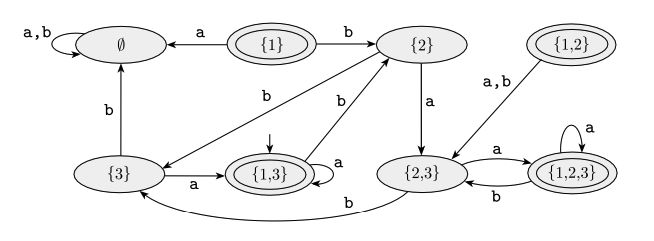
\includegraphics[width=\linewidth]{lecture05-dfa-equiv-of-nfa.png}

    The NFA's start state is $1$, so the DFA's start state is $E(\{1\})=\{1,3\}$ (the set of states reachable from $1$ by travelling along $\epsilon$ arrows and $1$ itself).
    The NFA's accepting state is $1$, so the DFA's accepting states are all sets of states that include $1$: $\{\{1\}, \{1,2\},\{1,3\},\{1,2,3\}\}$ \\

    As for $D$'s transition function, each of $D$'s states goes to one place on input $a$ and one place on input $b$ (by definition of DFA). We will illustrate a few.

    \begin{itemize}
        \item in $D$, state $\{2\}$ goes to $\{2,3\}$ on input $a$ because in $N$, state $2$ goes to both $2$ and $3$ on input $a$.
        \item in $D$, state $\{1\}$ goes to $\emptyset$ on input $a$ because no $a$ arrows exit it.
        \item in $D$, state $\{1,2\}$ goes to $\{2,3\}$ on input $a$ because in $N$, state $1$ goes nowhere on input $a$ and state $2$ goes to both $2$ and $3$ on input $a$
    \end{itemize}

    NFA with $n$ states $\rightarrow$ DFA with $2^n$ states.
\end{example}

\subsection{Closure Under Regular Operations}
\begin{theorem}
    The class of regular languages is closed under the union operation. \\

    \textit{Proof Idea.} We have regular languages $A_1$ and $A_2$ and want to prove that $A_1\cup A_2$ is regular.
    The idea is to take 2 NFAs, $N_1$ and $N_2$, that accept $A_1$ and $A_2$ respectively, and combine them into a single new NFA $N$.

    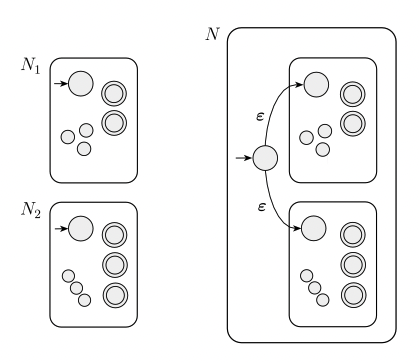
\includegraphics[width=\linewidth / 2]{lecture05-union-closure-nfa-proof-idea.png}
    \begin{proof}
        Let $N_1=(Q_1,\Sigma,\delta_1,q_1,F_1)$ recognize $A_1$ and $N_2=(Q_2,\Sigma,\delta_2,q_2,F_2)$ recognize $A_2$. \\

        Construct $N=(Q,\Sigma,\delta,q_0,F)$ to recognize $A_1\cup A_2$.

        \begin{enumerate}
            \item $Q=\{q_0\}\cup Q_1\cup Q_2$
            \subitem The states of $N$ are all the states of $N_1$ and $N_2$ with the addition of a new start state $q_0$.
            \item The state $q_0$ is the start state of $N$.
            \item The set of accepting states $F=F_1\cup F_2$.
            \subitem The accepting states of $N$ are all the accepting states of $N_1$ and $N_2$. That way, $N$ accepts if either $N_1$ or $N_2$ accepts.
            \item Define $\delta$ so that for any $q\in Q$ and any $a\in\Sigma_{\epsilon}$,
            $$\delta(q,a)=\begin{cases}
                \delta_1(q,a) & q\in Q_1 \\
                \delta_2(q,a) & q\in Q_2 \\
                \{q_1,q_2\} & q=q_0\text{ and }a=\epsilon \\
                \emptyset & q=q_0\text{ and }a\neq\epsilon
            \end{cases}$$
        \end{enumerate}
    \end{proof}
\end{theorem}

\begin{theorem}
    The class of regular languages is closed under the concatenation operation. \\

    \textit{Proof Idea.} We have regular languages $A_1$ and $A_2$ and want to prove that $A_1\circ A_2$ is regular.
    The idea is to take 2 NFAs, $N_1$ and $N_2$, and combine them into a single new NFA $N$ (like how we did in the union closure proof, but with a few changes).

    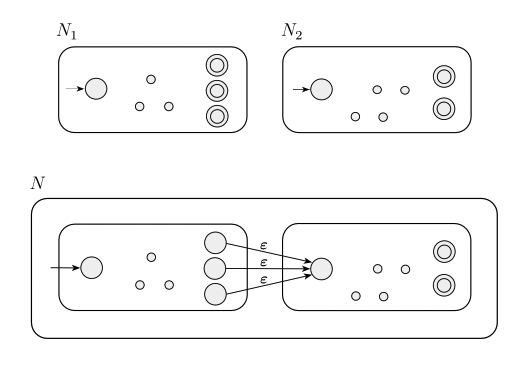
\includegraphics[width=\linewidth / 2]{lecture05-concat-closure-nfa-proof.png}

    \begin{proof}
        Let $N_1=(Q_1,\Sigma,\delta_1,q_1,F_1)$ recognize $A_1$ and $N_2=(Q_2,\Sigma,\delta_2,q_2,F_2)$ recognize $A_2$. \\

        Construct $N=(Q,\Sigma,\delta,q_0,F)$ to recognize $A_1\circ A_2$.

        \begin{enumerate}
            \item $Q=Q_1\cup Q_2$
            \subitem The states of $N$ are all the states of $N_1$ and $N_2$.
            \item The state $q_1$ is the start state of $N_1$.
            \item The set of accepting states $F_2$ are the same as the accepting states of $N_2$.
            \item Define $\delta$ so that for any $q\in Q$ and any $a\in\Sigma_{\epsilon}$,
            $$\delta(q,a)=\begin{cases}
                \delta_1(q,a) & q\in Q_1\text{ and }q\notin F_1 \\
                \delta_1(q,a) & q\in F_1\text{ and }a\neq\epsilon \\
                \delta_1(q,a)\cup\{q_2\} & q\in F_1\text{ and }a\in\epsilon \\
                \delta_2(q,a) & q\in Q_2
            \end{cases}$$
        \end{enumerate}
    \end{proof}
\end{theorem}

\begin{theorem}
    The class of regular languages is closed under the Kleene star operation. \\

    \textit{Proof Idea.} We have a regular language $A$ and want to prove that $A_1^*$ also is regular. We take an NFA $N_1$ for $A_1$ and modify it to recognize $A_1^*$ as shown.
    The resulting NFA $N$ will accept its input whenever it can be broken into several pieces and $N$ accepts each piece. \\

    We can construct $N$ like $N_1$ with additional $\epsilon$ arrows returning to the start state from the accepting states.
    This way when the processing gets to the end of a piece that $N_1$ accepts, the machine $N$ has the option of jumping back to the start state to try to read another piece that $N_1$ accepts.

    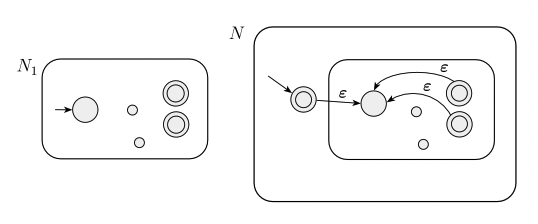
\includegraphics[width=\linewidth * 2 / 3]{lecture05-star-closure-nfa-proof.png}

    \begin{proof}
        Let $N_1=(Q_1,\Sigma,\delta_1,q_1,F_1)$ recognize $A_1$. Construct $N=(Q,\Sigma,\delta,q_0,F)$ to recognize $A_1^*$.

        \begin{enumerate}
            \item $Q=\{q_0\}\cup Q_1$
            \subitem The states of $N$ are the states of $N_1$ plus a new start state.
            \item The state $q_0$ is the new start state.
            \item $F=\{q_0\}\cup F_1$
            \subitem The accepting states are the old accepting states plus the new start state.
            \item Define $\delta$ so that for any $q\in Q$ and any $a\in\Sigma_{\epsilon}$,
            $$\delta(q,a)=\begin{cases}
                \delta_1(q,a) & q\in Q_1\text{ and }q\notin F_1 \\
                \delta_1(q,a) & q\in F_1\text{ and }a\notin\epsilon \\
                \delta_1(q,a)\cup\{q_1\} & q\in F_1\text{ and }a\in\epsilon \\
                \{q_1\} & q=q_0\text{ and }a\in\epsilon \\
                \emptyset & q=q_0\text{ and }a\notin\epsilon
            \end{cases}
            $$
        \end{enumerate}
    \end{proof}
\end{theorem}


% -----------------------------
% END OF LECTURE 5
% -----------------------------

% -----------------------------
% START OF LECTURE 6
% -----------------------------

\section{Lecture 6: Regular Expressions}
\subsection{Equivalence Of NFAs and DFAs (cont.)}
\begin{theorem}
    Every NFA has an equivalent DFA.

    \begin{proof}
        Let $N=(Q,\Sigma,\delta,q_0, F)$ be the NFA recognizing some language $A$. We construct DFA $M=(Q',\Sigma,\delta',q'_0,F')$ recognizing $A$.
        Before doing the full construction, first consider the easier case when $N$ has no $\epsilon$ arrows. We will take $\epsilon$ into account later.

        \begin{enumerate}
            \item $Q'=\mathcal{P}(Q)$ (the set of subsets of $Q$)
            \subitem Every state of $M$ is a set of states of $N$.
            \item $\Sigma$ (the alphabet) doesn't change
            \item For $R\in Q'$, and $a\in\Sigma$, let $\delta'(R,a)=\{q\in Q\mid q\in\delta(r,a)\text{ for some }r\in R\}$
            \subitem If $R$ is a state of $M$, it is also a set of states of $N$. When $M$ reads a symbol $a$ in state $R$, it shows where $A$ takes each state in $R$. Because each state may go to a set of states, we take the union of all these sets.
            $$\delta'(R,a)=\bigcup\limits_{r\in R}\delta(r,a)$$
            \item $q'_0=\{q_0\}$
            \subitem $M$ starts in the state corresponding to the collection containing just the start state of $N$.
            \item $F'=\{R\in Q'\mid R\text{ contains an accepting state of }N\}$
            \subitem The machine $M$ accepts if one of the possible states that $N$ could be in at this point is an accepting state.
        \end{enumerate}

        Now consider the $\epsilon$ arrows. For any state $R$ of $M$, we define $E(R)$ to be the collection of states that can be reached from members of $R$ by going only along $\epsilon$ arrows, including members of $R$ themselves.
        Formally, for $R\subseteq Q$, let $$E(R)=\{q\mid q\text{ can be reached from $R$ by traveling along 0 or more $\epsilon$ arrows}\}$$
        Then we modify the transition function of $M$ to place additional fingers on all states that can be reached by going along $\epsilon$ arrows after every step. Replacing $\delta(r,a)$ by $E(\delta(r,a))$ achieves this.
        Finally, we need to modify the start state of $M$ to move the fingers initially to all possible states that can be reached from the start state of $N$ along the $\epsilon$ arrows. \\
        
        The changes mentioned above to account for $\epsilon$ arrows are shown below:
        \begin{enumerate}
            \setcounter{enumi}{2}
            \item $\delta'(R,a)=\{q\in Q\mid q\in E(\delta(r,a))\text{ for some }r\in R\}$
            \item $q'_0=E(\{q_0\})$
        \end{enumerate}
    \end{proof}
\end{theorem}

\begin{example}
    Consider the following NFA $N$:

    \begin{tikzpicture}[node distance={2.5cm}, semithick, main/.style = {draw, circle}]
        \node[name=input] {};
        \node[state,accepting] (0) [right of=input] {$1$};
        \node[state] (1) [below of=0] {$2$};
        \node[state] (2) [right of=1] {$3$};

        % q_0
        \draw[->] (input) -- (0);
        \draw[->] (0) to node[left] {$b$} (1);
        \draw[->,out=295,in=155] (0) to node[above] {$\epsilon$} (2);

        % q_1
        \path (1) edge [loop left] node {$a$} (1);

        % q_2
        \draw[->,out=115,in=335] (2) to node[left] {0} (0);
        \draw[->] (1) to node[below] {$a,b$} (2);
    \end{tikzpicture}

    Note that the DFA will have 8 states, one for each subset of the states of $N$. The DFA and its transitions are shown below: \\

    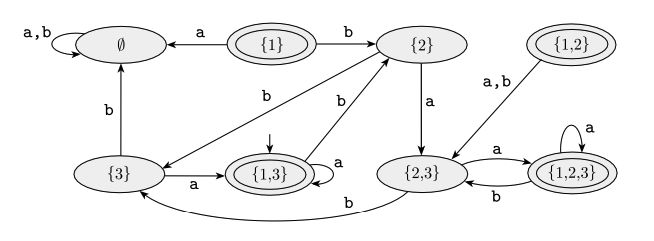
\includegraphics[width=\linewidth]{lecture05-dfa-equiv-of-nfa.png}

    The NFA's start state is $1$, so the DFA's start state is $E(\{1\})=\{1,3\}$ (the set of states reachable from $1$ by travelling along $\epsilon$ arrows and $1$ itself).
    The NFA's accepting state is $1$, so the DFA's accepting states are all sets of states that include $1$: $\{\{1\}, \{1,2\},\{1,3\},\{1,2,3\}\}$ \\

    As for $D$'s transition function, each of $D$'s states goes to one place on input $a$ and one place on input $b$ (by definition of DFA). We will illustrate a few.

    \begin{itemize}
        \item in $D$, state $\{2\}$ goes to $\{2,3\}$ on input $a$ because in $N$, state $2$ goes to both $2$ and $3$ on input $a$.
        \item in $D$, state $\{1\}$ goes to $\emptyset$ on input $a$ because no $a$ arrows exit it.
        \item in $D$, state $\{1,2\}$ goes to $\{2,3\}$ on input $a$ because in $N$, state $1$ goes nowhere on input $a$ and state $2$ goes to both $2$ and $3$ on input $a$
    \end{itemize}

    NFA with $n$ states $\rightarrow$ DFA with $2^n$ states.
\end{example}

\subsection{Closure Under Regular Operations}
\begin{theorem}
    The class of regular languages is closed under the union operation. \\

    \textit{Proof Idea.} We have regular languages $A_1$ and $A_2$ and want to prove that $A_1\cup A_2$ is regular.
    The idea is to take 2 NFAs, $N_1$ and $N_2$, that accept $A_1$ and $A_2$ respectively, and combine them into a single new NFA $N$.

    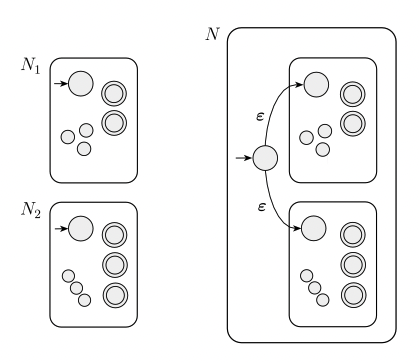
\includegraphics[width=\linewidth / 2]{lecture05-union-closure-nfa-proof-idea.png}
    \begin{proof}
        Let $N_1=(Q_1,\Sigma,\delta_1,q_1,F_1)$ recognize $A_1$ and $N_2=(Q_2,\Sigma,\delta_2,q_2,F_2)$ recognize $A_2$. \\

        Construct $N=(Q,\Sigma,\delta,q_0,F)$ to recognize $A_1\cup A_2$.

        \begin{enumerate}
            \item $Q=\{q_0\}\cup Q_1\cup Q_2$
            \subitem The states of $N$ are all the states of $N_1$ and $N_2$ with the addition of a new start state $q_0$.
            \item The state $q_0$ is the start state of $N$.
            \item The set of accepting states $F=F_1\cup F_2$.
            \subitem The accepting states of $N$ are all the accepting states of $N_1$ and $N_2$. That way, $N$ accepts if either $N_1$ or $N_2$ accepts.
            \item Define $\delta$ so that for any $q\in Q$ and any $a\in\Sigma_{\epsilon}$,
            $$\delta(q,a)=\begin{cases}
                \delta_1(q,a) & q\in Q_1 \\
                \delta_2(q,a) & q\in Q_2 \\
                \{q_1,q_2\} & q=q_0\text{ and }a=\epsilon \\
                \emptyset & q=q_0\text{ and }a\neq\epsilon
            \end{cases}$$
        \end{enumerate}
    \end{proof}
\end{theorem}

\begin{theorem}
    The class of regular languages is closed under the concatenation operation. \\

    \textit{Proof Idea.} We have regular languages $A_1$ and $A_2$ and want to prove that $A_1\circ A_2$ is regular.
    The idea is to take 2 NFAs, $N_1$ and $N_2$, and combine them into a single new NFA $N$ (like how we did in the union closure proof, but with a few changes).

    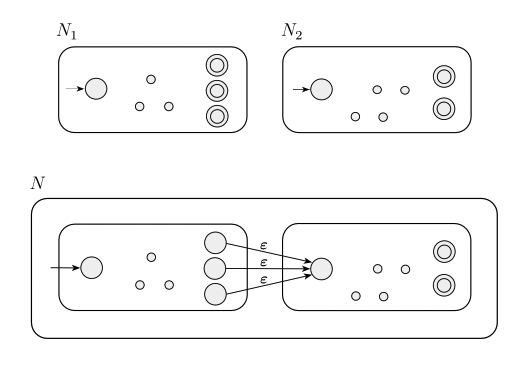
\includegraphics[width=\linewidth / 2]{lecture05-concat-closure-nfa-proof.png}

    \begin{proof}
        Let $N_1=(Q_1,\Sigma,\delta_1,q_1,F_1)$ recognize $A_1$ and $N_2=(Q_2,\Sigma,\delta_2,q_2,F_2)$ recognize $A_2$. \\

        Construct $N=(Q,\Sigma,\delta,q_0,F)$ to recognize $A_1\circ A_2$.

        \begin{enumerate}
            \item $Q=Q_1\cup Q_2$
            \subitem The states of $N$ are all the states of $N_1$ and $N_2$.
            \item The state $q_1$ is the start state of $N_1$.
            \item The set of accepting states $F_2$ are the same as the accepting states of $N_2$.
            \item Define $\delta$ so that for any $q\in Q$ and any $a\in\Sigma_{\epsilon}$,
            $$\delta(q,a)=\begin{cases}
                \delta_1(q,a) & q\in Q_1\text{ and }q\notin F_1 \\
                \delta_1(q,a) & q\in F_1\text{ and }a\neq\epsilon \\
                \delta_1(q,a)\cup\{q_2\} & q\in F_1\text{ and }a\in\epsilon \\
                \delta_2(q,a) & q\in Q_2
            \end{cases}$$
        \end{enumerate}
    \end{proof}
\end{theorem}

\begin{theorem}
    The class of regular languages is closed under the Kleene star operation. \\

    \textit{Proof Idea.} We have a regular language $A$ and want to prove that $A_1^*$ also is regular. We take an NFA $N_1$ for $A_1$ and modify it to recognize $A_1^*$ as shown.
    The resulting NFA $N$ will accept its input whenever it can be broken into several pieces and $N$ accepts each piece. \\

    We can construct $N$ like $N_1$ with additional $\epsilon$ arrows returning to the start state from the accepting states.
    This way when the processing gets to the end of a piece that $N_1$ accepts, the machine $N$ has the option of jumping back to the start state to try to read another piece that $N_1$ accepts.

    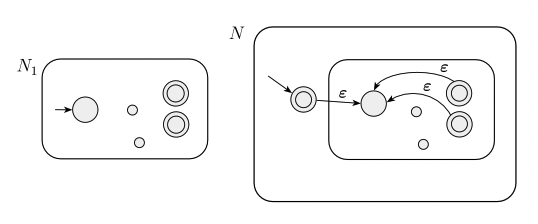
\includegraphics[width=\linewidth * 2 / 3]{lecture05-star-closure-nfa-proof.png}

    \begin{proof}
        Let $N_1=(Q_1,\Sigma,\delta_1,q_1,F_1)$ recognize $A_1$. Construct $N=(Q,\Sigma,\delta,q_0,F)$ to recognize $A_1^*$.

        \begin{enumerate}
            \item $Q=\{q_0\}\cup Q_1$
            \subitem The states of $N$ are the states of $N_1$ plus a new start state.
            \item The state $q_0$ is the new start state.
            \item $F=\{q_0\}\cup F_1$
            \subitem The accepting states are the old accepting states plus the new start state.
            \item Define $\delta$ so that for any $q\in Q$ and any $a\in\Sigma_{\epsilon}$,
            $$\delta(q,a)=\begin{cases}
                \delta_1(q,a) & q\in Q_1\text{ and }q\notin F_1 \\
                \delta_1(q,a) & q\in F_1\text{ and }a\notin\epsilon \\
                \delta_1(q,a)\cup\{q_1\} & q\in F_1\text{ and }a\in\epsilon \\
                \{q_1\} & q=q_0\text{ and }a\in\epsilon \\
                \emptyset & q=q_0\text{ and }a\notin\epsilon
            \end{cases}
            $$
        \end{enumerate}
    \end{proof}
\end{theorem}


% -----------------------------
% END OF LECTURE 6
% -----------------------------

% -----------------------------
% START OF LECTURE 7
% -----------------------------


\section{Lecture 7: Nonregular Languages}
\subsection{Example: Nonregular Language}
\begin{example}
    Consider the language $L=\{O^n1^n\mid n\geq 0\}$. \\

    If we attempt to find a DFA that recognizes $L$, we find that the machine needs to remember how many 0s have been read so far.
    Because the number of 0s is not limited, the machine will have to track an unlimited number of possibilities (but this can't be done with finite states).
    Therefore, $L$ is not a regular language.
\end{example}

\begin{example}
    Consider the language $A=\{w\mid w\text{ has an equal number of 0s and 1s}\}$ and $B=\{w\mid w\text{ has an equal number of occurrences of 01 and 10 as substrings}\}$.

    $A$ is not regular but $B$ is. Below, we will use the pumping lemma to show how to prove that certain languages are not regular.
\end{example}


\subsection{Pumping Lemma For Regular Languages}
\begin{theorem}
    If $A$ is a regular language, then there is a number $p$ (pumping length) where if $s$ is any string in $A$ of length $\geq p$, then $s$ may be divided into 3 pieces, $s=xyz$, satisfying the following conditions:
    \begin{itemize}
        \item for each $i\geq 0,xy^iz\in A$
        \item $|y|>0$
        \item $|xy|\leq p$
    \end{itemize}

    \begin{proof}
        If $A$ is regular then there exists a DFA $M$ accepting $A$. \\

        Let $M=(Q,\Sigma,\delta,q_1,F)$ be a DFA recognizing $A$ and $p$ be the number of states of $M$. \\

        Let $s=s_1s_2...s_n$ be a string in $A$ of length $n$, where $n\geq p$. Let $r_1,...,r_{n+1}$ be the sequence of states that $M$ enters while processing $s$, so $r_{i+1}=\delta(r_i,s_i)\text{ for }1\leq i\leq n$.
        This sequence has length $n+1$, which is at least $p+1$.
        Among the first $p+1$ elements in the sequence, 2 must be the same state, by the pigeonhole principle.
        Call the first of these $r_j$ and the second $r_l$. Because $r_l$ occurs among the first $p+1$ places in a seuqnce starting at $r_1$, we have $l\leq p+1$. \\

        Now let $x=s_1\cdots s_j-1,y=s_j\cdots s_{l-1},z=s_l\cdots s_n$. As $x$ takes $M$ from $r_1$ to $r_j$, $y$ takes $M$ from $r_j$ to $r_j$, and $z$ take s$M$ from $r_j$ to $r_{n+1}$, which is an accepting state so $M$ must accept $xy^iz\text{ for }i\geq 0$.
        We know that $j\neq l$, so $|y|>0$, and $l\leq p+1$, so $|xy|\leq p$, and have satisfied all conditions of the pumping lemma. \\
    \end{proof}
\end{theorem}

\subsubsection{Examples: Using Pumping Lemma To Prove Nonregularity}
\begin{example}
    Consider the language $B$ be the language $\{0^n1^n\mid n\geq 0\}$.

    \begin{proof}
        Assume that $B$ is regular. \\
        
        Let $p$ be the pumping length given by the pumping lemma.
        Choose $s$ to be a string $0^p1^p$. Because $s$ is a member of $B$ and $s$ has length more than $p$, the pumping lemma guarantees that $s$ can be split into 3 pieces, $s=xyz$, where for any $i\geq 0$ the string $xy^iz$ is in $B$.
        Let us consider 3 cases to show that this result is impossible:

        \begin{enumerate}
            \item The string $y$ consists only of $0$s. For example, $xyyz$ (when $i=2$) has more $0$s than $1$s, so it is in the language $B$. This breaks condition 1 of the pumping lemma.
            \item The string $y$ consists only of $1$s. This also breaks condition 1.
            \item The string $y$ consists of both $0$s and $1$s. The string $xyyz$ may have the same number of $0$s and $1$s, but they are out of order. So the string is not in $B$ and breaks condition 1 of the pumping lemma.
        \end{enumerate}
    \end{proof}
\end{example}

\begin{example}
    Let $C=\{w\mid w\text{has an equal number of $0$s and $1$s}\}$. Prove that $C$ is not regular.

    \begin{proof}
        Assume that $C$ is regular. \\

        Let $p$ be the pumping length given by the pumping lemma. Choose $s$ to be the string $0^p1^p$.
        Because $s$ is a member of $C$ and $s$ has length more than $p$, the pumping lemma guarantees that $s$ can be split into 3 pieces, $s=xyz$, where for any $i\geq 0$ the string $xy^iz$ is in $C$. \\
        
        Let $x$ and $z$ be the empty string and $y$ be the string $0^p1^p$. Then $xy^iz$ always has an equal number of $0$s and $1$s and is in $C$. \\

        BUT THIS IS WRONG! CONDITION 3 OF THE PUMPING LEMMA COMES INTO PLAY. \\
        
        By pumping $s$, it must be divided so that $|xy|\leq p$. That means the string we selected $s=0^p1^p$ cannot be pumped.
        If $|xy|\leq p$, then $y$ must consist only of $0$s, so $xyyz\notin C$. \\

        $s$ cannot be pumped and therefore $C$ is not regular. \\
    \end{proof}
\end{example}

\begin{example}
    Consider the language $D=\{ww\mid w\in\{0,1\}^*\}$. Prove that $D$ is not regular.
    
    \begin{proof}
        Assume that $F$ is regular. \\

        Let $s$ be the string $0^p10^p1$. Because $s$ is a member of $F$ and $s$ has length more than $p$, the pupming lemma guarantees that $s$ can be split into 3 pieces $s=xyz$ satisfying the pumping lemma. \\

        Condition 3 of the pumping lemma is important again. We cannot let $x$ and $z$ be of length 0 because of condition 3.
        This means that $y$ must consist of only $0$s, so $xyyz\notin D$. \\
    \end{proof}
\end{example}

\begin{example}
    Consider the language $\tilde{L_3}=\{w_1w_2\mid w_1\neq w_2;w_1,w_2\in \Sigma^*\}$. \\

    Then $L_3=(\Sigma\Sigma)^*-\tilde{L_3}=(\Sigma\Sigma)^*\cap \tilde{L_3}$
\end{example}

\subsubsection{Example: Pumping Lemma On Unary Languages}
\begin{example}
    Consider the language $E=\{1^{n^2}\mid n\geq 0\}$. $E$ essentially contain all strings of 1s whose lengths is a perfect square. We will show that $E$ is not regular. \\

    \begin{proof} By contradiction: \\

        Assume that $E$ is regular. Let $p$ be the pumping length given by the pumping lemma. Let $s$ be the string $1^{p^2}$.
        Because $s$ is a member of $E$ and $s$ has length at least $p$, the pumping lemma guarantees that $s$ can be split into $s=xyz$, where for any $i\geq 0$, the string $xy^iz$ is in $D$. \\

        Consider the 2 strings $xyz$ and $xy^2z$. These strings differ from each other by a single repetition of $y$ and their lengths differ by the length of $y$. By condition 3 of the pumping lemma, $|xy|\leq p$ and thus $|y|\leq p$.
        We have $|xyz|=p^2$ and so $|xy^2z|\leq p^2+p$. But $p^2+p<p^2+2p+1=(p+1)^2$. Condition 2 implies that $y$ is not an empty string so $|xy^2z|>p^2$. The length of $xy^2z$ lies strictly between the consecutive perfect squares $p^2$ and $(p+1)^2$.
        So the length cannot be a perfect square, see that $xy^2z\notin E$, and conclude that $E$ is not regular. \\
    \end{proof}
\end{example}

\subsubsection{Example: Pumping Down}
\begin{example}
    Consider the language $F=\{0^j1^j\mid i>j\}$. Show that $F$ is not regular.

    \begin{proof}
        Assume that $F$ is not regular. \\

        Let $p$ be the pumping length of $F$ given by the pumping lemma. By condition 3, $y$ consists only of $0$s.
        Let's example the string $xyyz$ to see whether it can be in $F$. Adding an extra copy of $y$ increases the number of $0$s.
        But $F$ contains all strings in $0^*1^*$ that have more $0$s and $1$s, so increasing the number of $0$s will still give the string in $F$.
        There is no contradiction. Try the following. \\

        The pumping lemma states that $xy^iz\in F$ even when $i=0$, so let's consider the string $xy^0z=xz$.
        Removing string $y$ decreases the number of $0$s in $s$. Remember than $s$ has just one more $0$ than $1$.
        Therefore, $xz$ cannot have more $0$s than $1$s, so it cannot be a member of $F$. This is a contradiction. \\
    \end{proof}
\end{example}


% -----------------------------
% END OF LECTURE 7
% -----------------------------

% -----------------------------
% START OF LECTURE 8
% -----------------------------


\section{Lecture 8: Context-Free Languages (CFLs)}
\subsection{Context-Free Grammars (CFGs)}
\begin{itemize}
    \item A grammar consists of collection of \textbf{substitution rules}, called \textbf{productions}.
    \item Each rule appears as a line in the grammar, comprising a symbol and a string separated by an arrow
    \item The symbol is called a \textbf{variable}.
    \item The string consists of variables and other symbols called \textbf{terminals}.
    \item The variables are often represented by capital letters. The terminals are often represented by lowercase letters, numbers, or special symbols.
    \item One variable is designated as the \textbf{start variable}.
\end{itemize}

You use a grammar to describe a language by generating each string of that language in the following manner.
\begin{enumerate}
    \item Write down the start variable. It is the variable on the left-hand side of the top rule, unless specified otherwise.
    \item Find a variable that is written down and a rule that starts with that variable. Replace the written down variable with the right-hand side of that rule.
    \item Repeat step 2 until no variables remain. \\
\end{enumerate}

\begin{example}
    Consider the grammar $G_1$:
    \begin{align*}
        A & \rightarrow 0A1 \\
        A & \rightarrow B \\
        B & \rightarrow\#
    \end{align*}

    \begin{itemize}
        \item $0,1,\#$ are terminals
        \item let $A$ be the start symbol
        \item $A\rightarrow 0A1\rightarrow 00A11\rightarrow 000B111\rightarrow 000\#111$ is a derivation
        \item $000\#111$ is a string of terminals
    \end{itemize}

    We can say that $G_1$ generates $0^3\#1^3$. \\

    Define $L(G)$ to be all strings generated by $G$. We can prove $L(G_1)=\{0^n\#1^n\mid n\geq 0\}$. Then $L(G_1)$ is a CFL because it is generated by a CFG.
    We say that $S=000\#111\in L(G_1).$ \\

    The following is a parse tree that describes the derivation of $S$.

    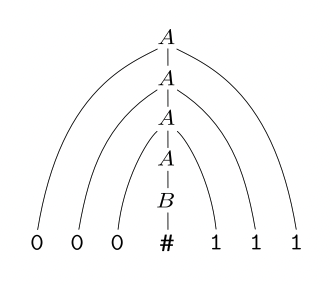
\includegraphics[width=\linewidth / 2]{lecture08-g1-parse-tree.png}

    Pulling all the leaves from the tree (shown by thin lines), we can see the string that is generated.
    Every word that is generated/derived from the start state has a parse tree.
    Grammars and parse tress come from linguistics. \\

    For example, English has a grammar and can be parsed.
\end{example}

\newpage
\subsubsection{Formal Definition Of A Context-Free Grammar}
\begin{definition}
    A \textbf{context-free grammar} is a 4-tuple $(V,\Sigma,R,S)$, where:
    \begin{itemize}
        \item $V$ is a finite set called the \textbf{variables}
        \item $\Sigma$ is a finite set, disjoint from $V$, called the \textbf{terminals}
        \item $R$ is a finite set of \textbf{rules}, with each rule being a variable and a string of variables and terminals, shown below
        $$\text{variable}\rightarrow\text{string}$$
        \item $S\in V$ is the start variable
    \end{itemize}
\end{definition}

If $u,v,w$ are strings of variables and terminals, and $A\rightarrow w$ is a rule of the grammar, we say that $uAv$ yields $uwv$, written $uAv\Rightarrow uwv$.
Say that $u\text{ derives } v$, written $u\Rightarrow v$, if $u=v$ or if a sequence $u_1,u_2,...,u_k$ exists for $k\geq 0$ and $$u\Rightarrow u_1\Rightarrow ...\Rightarrow u_k\Rightarrow v$$ \\


\begin{example}
    Consider the grammar $G_2=(\{S\},\{a,b\}R,S)$. The set of rules $R$ is $$S\rightarrow aSb\mid SS\mid\epsilon$$

    This grammar generates strings such as $abab$, $aaabbb$, and $aabaab$.
    Think of $a$ as '(' and $b$ as ')'. Viewed in this way, $L(G_3)$ is the language of all strings of properly nested (balanced) parentheses.
    Note that the language may contain the empty string $\epsilon$.
\end{example}

\begin{example}
    Consider the grammar $G_3=(V,\Sigma,R,\langle EXPR\rangle)$. \\

    $V$ is $\{\langle EXPR\rangle,\langle TERM\rangle,\langle FACTOR\rangle\}$ and $\Sigma$ is $\{a,+,\times, (, )\}$
    \begin{align*}
        \langle EXPR\rangle &\rightarrow\langle EXPR\rangle+\langle TERM\rangle\mid\langle TERM\rangle \\
        \langle TERM\rangle &\rightarrow\langle TERM\rangle\times\langle FACTOR\rangle\mid\langle FACTOR\rangle \\
        \langle FACTOR\rangle &\rightarrow (\langle EXPR\rangle)\mid a
    \end{align*}

    The two strings $a+a\times a$ and $(a+a)\times a$ are both generated with grammar $G_3$. The parse trees are shown below:

    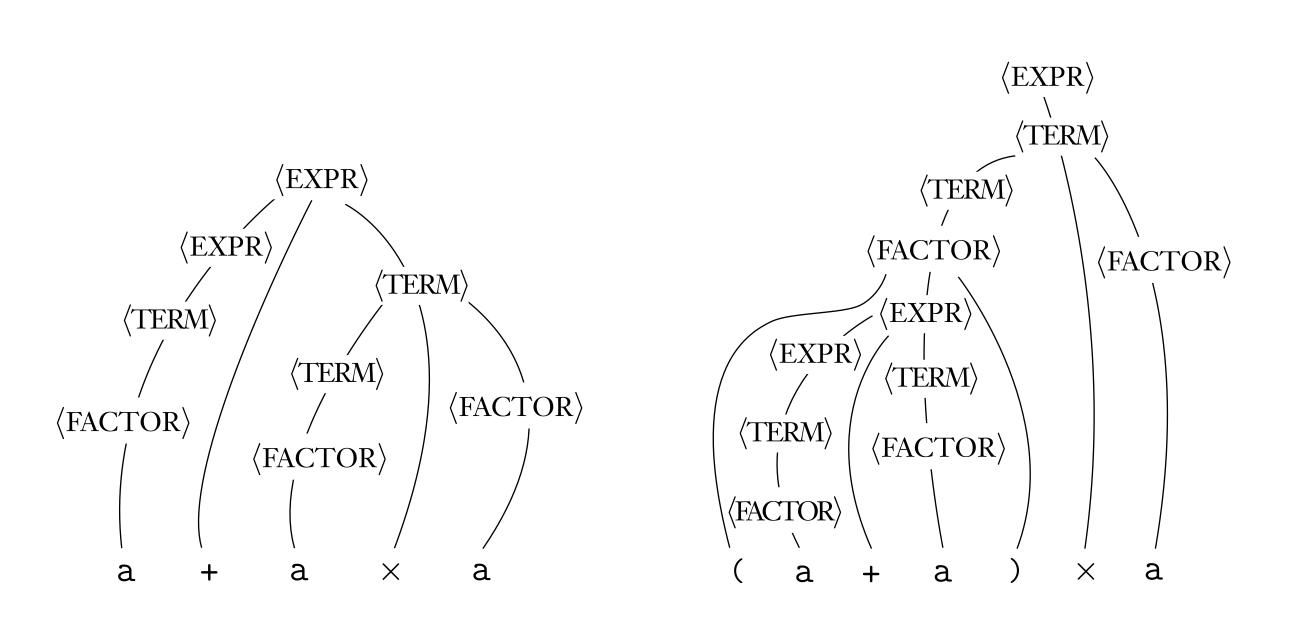
\includegraphics[width=\linewidth]{lecture08-g3-ex.png}
\end{example}

\subsubsection{Designing Context-Free Grammars}

Many CFLs are unions of simpler CFLs. \\

\begin{example}
    To get a grammar for the language $\{0^n1^n\mid n\geq 0\}\cup \{1^n0^n\mid n\geq 0\}$, first construct the grammar. \\

    $S_1\rightarrow 0S_1 1\mid\epsilon$ for language $\{0^n1^n\mid n\geq 0\}$
    $S_2\rightarrow1S_2 0\mid\epsilon$ for language $\{1^n0^n\mid n\geq 0\}$ \\

    Then add the rule $S\rightarrow S_1\mid S_2$ to give the grammar:
    \begin{align*}
        S &\rightarrow S_1\mid S_2 \\
        S_1 &\rightarrow 0S_1 1\mid\epsilon \\
        S_2 &\rightarrow 1S_2 0\mid\epsilon
    \end{align*}
\end{example}

Constructing a CFG for a language that happens to be regular is easy if you can first construct a DFA for that language.
You can convert any DFA into an equivalent CFG by:
\begin{enumerate}
    \item Make a variable $R_i$ for each state $q_i$ of the DFA.
    \item Add the rule $R_i\rightarrow aR_j$ to the CFG if $\delta(q_i,a)=q_j$ is the transition in the DFA.
    \item Add the rule $R_i\rightarrow\epsilon$ if $q_i$ is an accepting state of the DFA.
    \item Make $R_0$ the start variable of the grammar, where $q_0$ is the start state of the machine
\end{enumerate}

Certain CFLs contain strings with two substrings that are "linked" in the sense that a machine for such a language would need to remember an unbounded amount of information about one of the substrings to verify that it corresponds properly to the other substring. \\

\begin{example}
    Consider the language $\{0^n1^n\mid n\geq 0\}$. \\

    The machine would need to remember the number of 0s in order to verify that it equals the number of 1s.
    You can construct a CFG to handle this situation by using a rule of the form $R\rightarrow uRv$, which generates strings wherein the portion containing the $u$'s correspond to the portion containing the $v$'s.
\end{example}


In more complex languages, the strings may contain certain structures that appear recursively as part of other (or the same) structures.
An example is Example 3, where the grammar generates arithmetic expressions. Any time a symbol $a$ appears, an entire parenthesized expression might appear recursively instead.
To do this, put the variable symbol generating the structure in the location of the rules corresponding to where that structure may recursively appear.


\subsubsection{Nondeterminism With CFGs}
CFGs are in some sense nondeterministic because at each step, we can choose:
\begin{enumerate}
    \item which rule to apply
    \item which variable to apply the rule
\end{enumerate}

\begin{example}
    Consider the string $0AB1A0$. \\

    We can eliminate nondeterminism for (2) with leftmost derivation (applying the rule to the leftmost variable).
    However we cannot entirely eliminate nondeterminism because there can be multiple choices for the rule from a variable such as $A\rightarrow w_1\mid w_2\mid w_3\mid w_4$.
\end{example}

\subsubsection{Ambiguity}
If the grammar generates the same string in several ways, we say that the string is derived \textbf{ambiguously}.
If a grammar generates some string ambiguously, we say that the grammar is \textbf{ambiguous}. \\

More formally, if $w\in L(G)$, then $S\stackrel{*}{\Rightarrow}w$. Sometimes $S\stackrel{*}{\Rightarrow}w$ in more than 1 way, and if this happens with $G$, then $G$ is ambiguous. \\

\begin{example}
    Let $L=\{a^ib^jc^k\mid i=j\text{ or }j=k\}$. \\

    It can be shown that $L$ is generated by a CFG, and $L$ is inherently ambiguous. Consider the following grammar $G_5$ for $L$:
    \begin{align*}
        S & \rightarrow S_1C\mid AS_2 \\
        S_1 & \rightarrow aS_1b\mid\epsilon \\
        S_2 & \rightarrow bS_2c\mid\epsilon \\
        A & \rightarrow aA\mid\epsilon \\
        C & \rightarrow Cc\mid\epsilon \\
    \end{align*}

    A string such as $aabbcc$ can be generated through multiple different paths.
\end{example}

\begin{example}
    Consider grammar $G_4=(V,\Sigma,R,\langle EXPR\rangle)$.

    $$\langle EXPR\rangle\rightarrow \langle EXPR\rangle+\langle EXPR\rangle\mid\langle EXPR\rangle\times\langle EXPR\rangle\mid (\langle EXPR\rangle)\mid a$$

    The following is two parse trees for the string $a+a\times a$ in grammar $G_4$.

    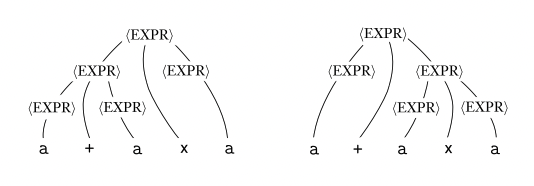
\includegraphics[width=\linewidth]{lecture08-g4-ex.png}

    Note that grammar $G_4$ does not capture the usual precedence relations ($\times$ before +).
\end{example}


% -----------------------------
% END OF LECTURE 8
% -----------------------------



\end{document}